\documentclass{article}

\usepackage{amsmath,bm}
\usepackage{amssymb}
\usepackage{amsfonts}
\usepackage[usenames]{xcolor}
\usepackage{graphicx}
\usepackage{epsf}
\usepackage{hyperref}
\usepackage{enumitem}

\usepackage[LGR,T1,OT1]{fontenc}
% \usepackage[sfdefault]{FiraSans}
% \usepackage[nomap]{FiraMono}
% \usepackage[var0,varqu]{zi4}
% \renewcommand{\rmdefault}{zi4}
%\renewcommand{\sfdefault}{zi4}

\usepackage[scaled=1.15]{newtxtext,newtxmath}
\usepackage{sansmathfonts}
% \usepackage{GoSans}
% % \renewcommand*\familydefault{\sfdefault} %% Only if the base font of the document is to be sans serif

% \usepackage{mathpazo}
% \usepackage{domitian}
% \usepackage[T1]{fontenc}
% \let\oldstylenums\oldstyle
%\usepackage{mathptmx}



\usepackage{unicode}

% titlepage causes separate title page
% our latex is biased off 1in vertically and horizontally
\newtheorem{theorem}{Theorem}
\setlength{\topmargin}{0.1in}
\setlength{\oddsidemargin}{0in}
\setlength{\evensidemargin}{0in}
\setlength{\headheight}{0in}
\setlength{\headsep}{0in}
\setlength{\textheight}{9in}
\setlength{\textwidth}{6.5in}
% require that floats fill 90% of a page in order for that page to be
% ``float-only''
\renewcommand{\dblfloatpagefraction}{0.9}
\renewcommand{\floatpagefraction}{0.9}
\newenvironment{bibparagraph}{\begin{list}{}{ %
    \setlength{\labelsep}{-\leftmargin} %
    \setlength{\labelwidth}{0pt} %
    \setlength{\itemindent}{-\leftmargin} %
    \setlength{\listparindent}{0pt}}}{\end{list}}
\def\makefigure#1#2{\begin{figure}
\begin{center}
\input{#1}
\end{center}
\caption{#2}%
\label{#1}
\end{figure}}

\def\limplies{\;\supset\;}
\def\land{\:\wedge\:}
\def\lor{\:\vee\:}
\def\iff{\;\equiv\;}
\def\lnot{\neg}
\def\lforall#1{\forall\: #1 \;}
\def\lexists#1{\exists\: #1 \;}
\def\glitch#1{{\tt #1}} % glitch on
%\def\glitch#1{} % glitch off
\def\comment#1{}
\def\pnil{[\;]}
\def\pif{\; \mbox{\tt:- } \;}
\def\tuple#1{$\langle#1\rangle$}
\def\mtuple#1{\langle#1\rangle}
\def\ceiling#1{\lceil#1\rceil}
\def\floor#1{\lfloor#1\rfloor}
\def\centerps#1{\begin{center}
\leavevmode
\epsfbox{#1}
\end{center}}
\def\argmax{\mathop{\rm argmax}}
\def\argmin{\mathop{\rm argmin}}
\def\grad{\nabla\!}
\def\celsius{^\circ\mbox{C}}
%\long\def\answer#1{}  % comment out for solutions
%\long\def\question#1{#1} % comment out for solutions
\long\def\answer#1{{\sf \noindent \color{blue!90!black!99!} \fontsize{11pt}{13.2pt}\selectfont #1} \vspace{2ex}}  % comment in for solution
\long\def\question#1#2{\rm \noindent {#1}. \color{black!99!}{{#2}} \par \vspace*{2ex}
} % comment in for solution
%\renewcommand{\labelenumi}{(\alph{enumi})}
%\newcommand{\mbx}{\mathbf{x}}
\newcommand{\mb}[1]{{\mathbf{#1}}}

\def\x{{\bf x}}
\def\w{{\bf w}}
\def\y{{\bf y}}

\usepackage{array}
\def\arraystretch{1.2}%
\linespread{1.5}

\usepackage{multirow}

\begin{document}

{\small
Submitted by: {Oluwasegun Somefun}, somefuno@oregonstate.edu
}
{\Large
\begin{center}
  AI534 ---  IA4 Homework Report {Due Dec 3rd 11:59pm, 2021}
\end{center}
}

\section{Introduction}

This report is on Decision Tree and Ensembles for Mushroom Classification, with respect to the Implementation Assignment 4.

\noindent \emph{Team Name}: Oluwasegun Ayokunle Somefun

\section{Part 1: Decision Tree (50pts)}
\question{a}{
  What are the first three splits selected by your algorithm? This is for the root, and the two splits
  immediately beneath the root. What are their respective information gains?
}
\answer{
The first 3 splits selected by the decision algorithm using maximum mutual information gain split criterion are highlighted in Table~\ref{taba}.
\begin{table}[!ht]
  \fontsize{10}{10} \centering \sf 
  \caption{First 3 node splits}
  \vspace{2ex}
  \begin{tabular}{|c|c|>{\bfseries}c|c|}
    \hline
    \textbf{Node} & \textbf{feature} & information gain \\ \hline\hline
    Root Split         & odor=n   & 0.54 \\\hline
    True Branch Split  & bruises?=f   & 0.4  \\\hline
    False Branch Split & spore-print-color=r   & 0.1  \\\hline
  \end{tabular}
  \label{taba}
\end{table}

}

\question{b}{
  Evaluate and plot the training and validation accuracies of your trees as a function of $d_{\max}$ ranging
  from 1 to 10. At which depth does the train accuracy reaches to 100\%? Do you observe any overfitting?
}
\answer{
\begin{figure}[!ht]
  \centering
  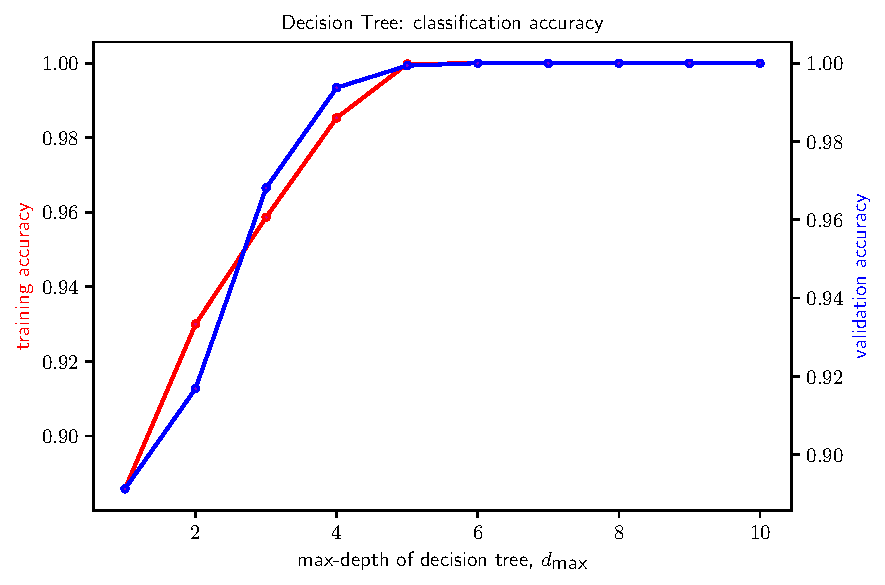
\includegraphics[width=0.6\linewidth]{figs/figtree_pt1.pdf}
  \caption{ Decision Tree: training/validation class accuracies as a function of maximum depth}\label{figb}
\end{figure}
At depth $d_{\max}=6$, the train accuracy reaches $100\%$. This together with the validation accuracy of $100\%$ is reported in Figure~\ref{taba}. 
Technically, there was no observation of overfitting, since the validation accuracy does not reduce even as $d_{\max}>6$ increases. However, this would imply overtraining, which could lead to overfitted decisions, depending on the data distribution.
}


\section{Part 2: Random Forest (35pts)}
\question{a}{ For each $d_{\max}$ value, create two figures, one for training accuracy and one for validation accuracy. The training accuracy figure should contain four curves, each showing the train accuracy of your random forest with a particular $m$ value as a function of $T$. Repeat the same process for validation accuracy. 

  Compare your training curves with the validation curves, do you think your model is overfitting or underfitting for particular parameter
  combinations? And why?
}
\answer{
  The training curves and validation curves are oultined in Figures~\ref{fig2a1}--\ref{fig2a6}. Comparing both curves, we see that for each maximum depth $d_{\max}$ the model performance of the random forest was not consistent and depended more on the number of random subsampled features $m$ compared to the increase in the number of trees $T$ in the forest ensemble. Also, we observe that as expected, both train and validation curves behave similarly, hence indicating random forest leads to low variance models but needs low bias models as base learners. This can be easily observed from the accuracy curves. Specifically, an additional value of $m$ was also added to account for subsampling using the total feature population $117$.
  \begin{figure*}[!ht]
    \centering
    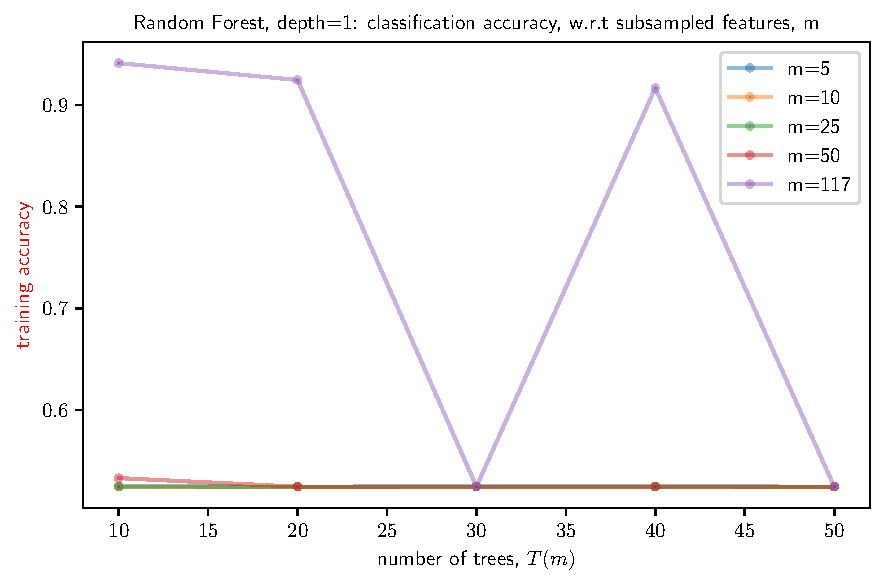
\includegraphics[width=0.5\linewidth]{figs/figforest_1_pt2_train.pdf}
    \caption{Random Forest $d_{\max}=1$: Training accuracy}\label{fig2a1}
  \end{figure*}
  \begin{figure*}[!ht]
    \centering
    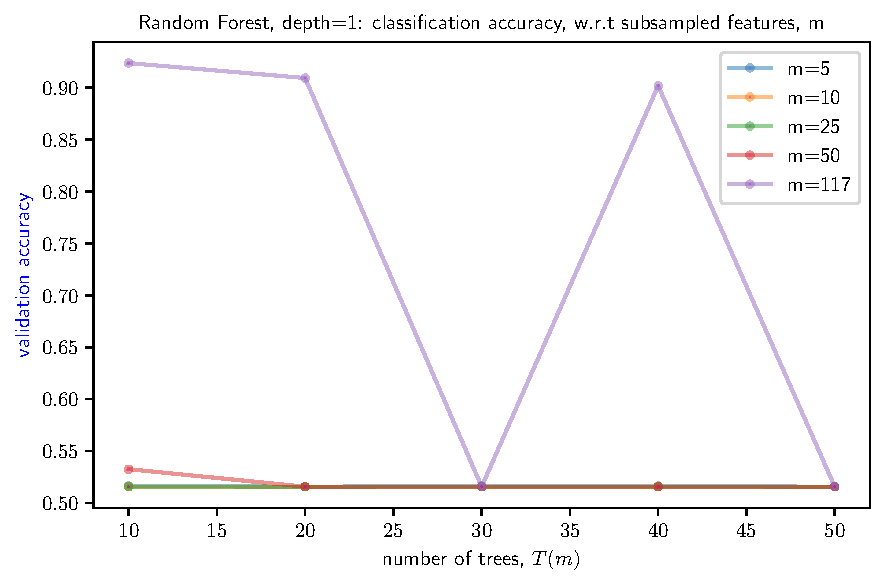
\includegraphics[width=0.5\linewidth]{figs/figforest_1_pt2_dev.pdf}
    \caption{Random Forest $d_{\max}=1$: Validation accuracy}\label{fig2a2}
  \end{figure*}
  \begin{figure*}[!ht]
    \centering
    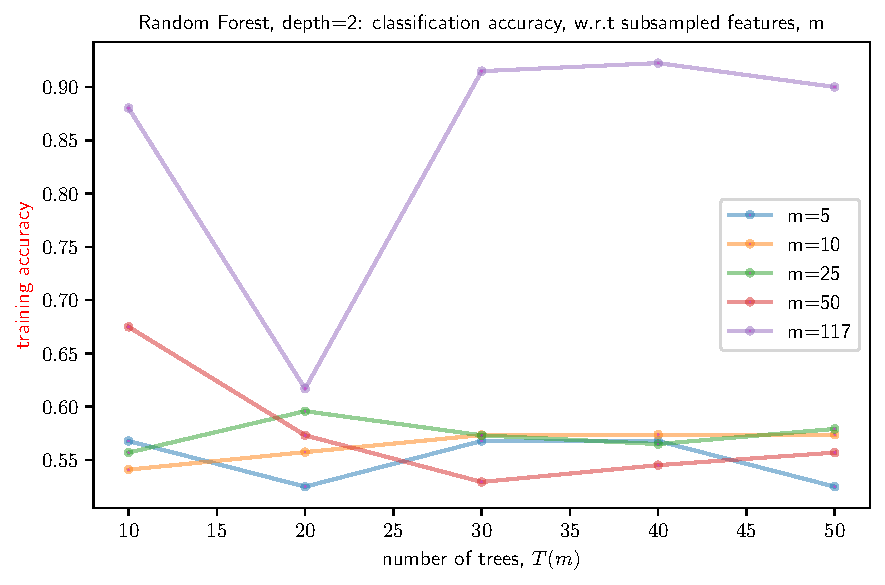
\includegraphics[width=0.5\linewidth]{figs/figforest_2_pt2_train.pdf}
    \caption{Random Forest $d_{\max}=2$: Training accuracy}\label{fig2a3}
  \end{figure*}
  \begin{figure*}[!ht]
    \centering
    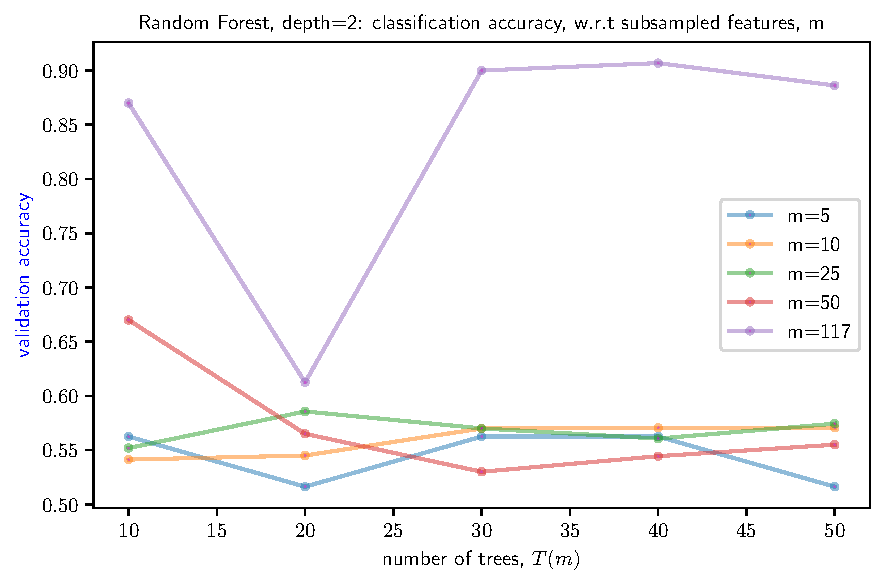
\includegraphics[width=0.5\linewidth]{figs/figforest_2_pt2_dev.pdf}
    \caption{Random Forest $d_{\max}=2$: Validation accuracy}\label{fig2a4}
  \end{figure*}
  \begin{figure*}[!ht]
    \centering
    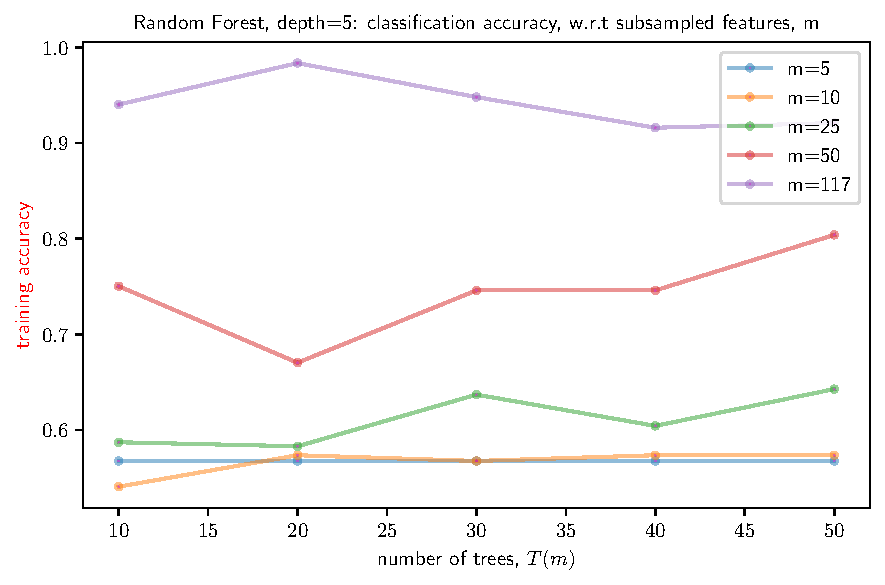
\includegraphics[width=0.5\linewidth]{figs/figforest_5_pt2_train.pdf}
    \caption{Random Forest $d_{\max}=5$: Training accuracy}\label{fig2a5}
  \end{figure*}
  \begin{figure*}[!ht]
    \centering
    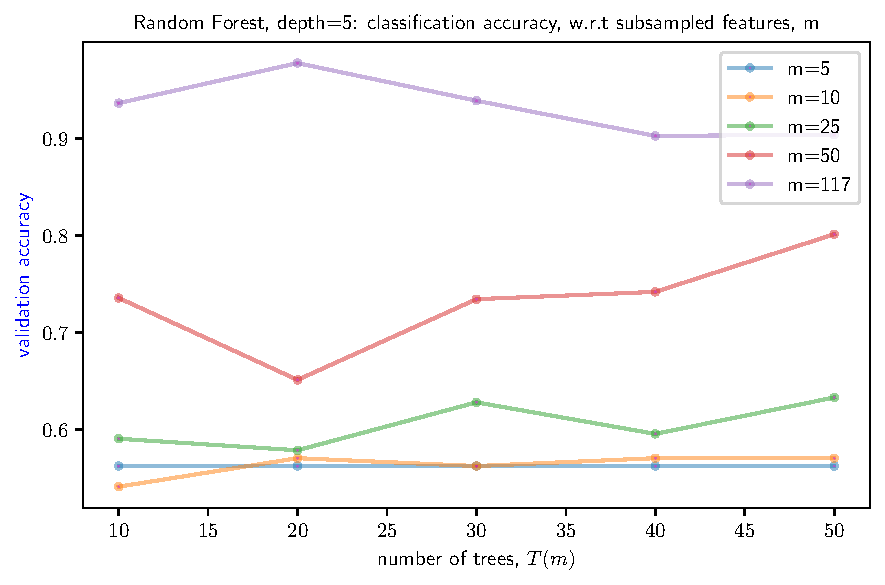
\includegraphics[width=0.5\linewidth]{figs/figforest_5_pt2_dev.pdf}
    \caption{Random Forest $d_{\max}=5$: Validation accuracy}\label{fig2a6}
  \end{figure*}
  
  For $d_{\max}=1$, see Figures~\ref{fig2a1}--\ref{fig2a2}, observe that the model, although of low variance, generally underfits the data for all $m$ as the number of trees $T>10$ is increased. 

  For $d_{\max}=2$, see Figures~\ref{fig2a3}--\ref{fig2a4}, observe that as $m$ increases the model accuracy improves on the data better than the previous depth.

  For $d_{\max}=5$, Figures~\ref{fig2a5}--\ref{fig2a6} show that as $m$ increases the range of model accuracy improves on the data better than the previous lower  mamxium depths.

}

\question{b}{
  For each $d_{\max}$ value, discuss what you believe is the dominating factor in the performance loss based on the concept of bias-variance decomposition. Can you suggest some alternative configurations of
  random forest that might lead to better performance for this data? Why do you believe so?
}
\answer{
  \begin{table}[!ht]
    \fontsize{10}{10} \centering \sf 
    \caption{mean out-of-bag (OOB) accuracy estimates}
    \vspace{2ex}
    \begin{tabular}{|c|c|c|c|c|c|}
      \hline
      \multirow{2}{*}{$d_{\max}$} & \multicolumn{5}{c|}{$m$}\\\cline{2-6}
        & 5 &10 &25 &50 &117\\\hline\hline
      1 & 0.52 & 0.53 & 0.54 & 0.55 & 0.60\\\hline
      2 & 0.53 & 0.55 & 0.57 & 0.57 & 0.67\\\hline
      5 & 0.55 & 0.56 & 0.61 & 0.62 & 0.80 \\\hline
    \end{tabular}
    \label{tabb}
  \end{table}
  It was observed that generally, for each $d_{\max}$ as $m$ increases, the mean out-of-bag (OOB) estimate (see Table~\ref{tabb}) for each ensemble configuration increases. For $d_{\max} = 1$, irrespective of $m$ and $T$, the model has the highest bias, and a low variance. For $d_{\max} = 2$, variance is low and as $m$ increases, the bias error generally reduces, although the behaviour is unstable as $T$ is increased. For $d_{\max} = 5$, again the variance is low, but this configuration has the lowest bias error compared to the previous depths.

  It can bes seen that for this dataset, to obtain better performance with lower bias error, $d_{\max}$ should be set to a suitable value that allows the base tree learner to be strong. Also, the number of sub-sampled features with replacement $m$, in the \textbf{Random forest} should be increased close to the full or total number of features in this data-set, that is: $m=117$.
}



\section{Bonus Part 3: AdaBoost (20pts) and Kaggle competition (5pts)}
\question{a}{
  For each $d_{\max}$ value, create a figure showing two curves, showing the accuracy (y-axis) on train and
  validation of your ensemble as a function of $T$. Repeat the same process for validation accuracy. 

  Compare your training curves with the validation curves, do you think your model is overfitting or underfitting for particular parameter
  combinations? And why?

}
\answer{
  Comparing the training curves with the validation curves in Figures~\ref{fig3a1}-\ref{fig3a3}, neither underfitting nor overfitting can be observed. This is clearly seen as the training and validation accuracies are similar. 
  
  This behaviour is expected in boosting, since boosting leads to decision-tree models with a lower bias and lower variance. However, overtraining can be observed as the number of trees in the ensemble increase.
\begin{figure}[!ht]
    \centering
    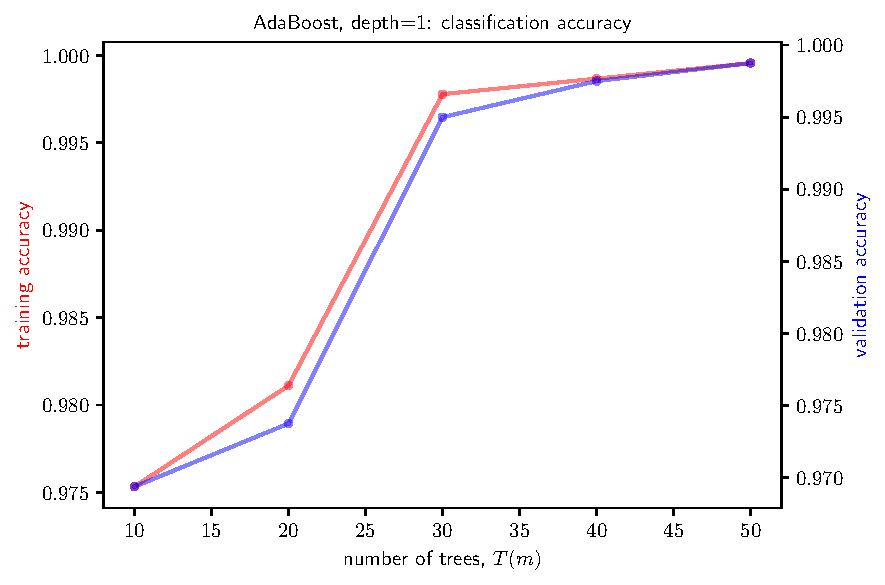
\includegraphics[width=0.6\linewidth]{figs/figadaboost_1_pt3_traindev.pdf}
    \caption{Adaboost: Train and validaition curves for $d_{\max}=1$}\label{fig3a1}
\end{figure}
\begin{figure}[!ht]
  \centering
  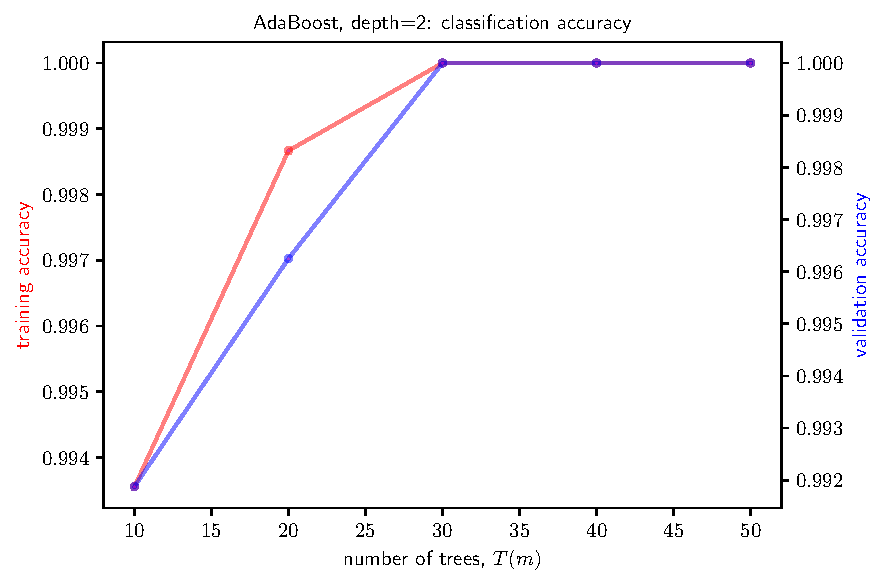
\includegraphics[width=0.6\linewidth]{figs/figadaboost_2_pt3_traindev.pdf}
  \caption{Adaboost: Train and validaition curves for $d_{\max}=2$}\label{fig3a2}
\end{figure}
\begin{figure}[!ht]
  \centering
  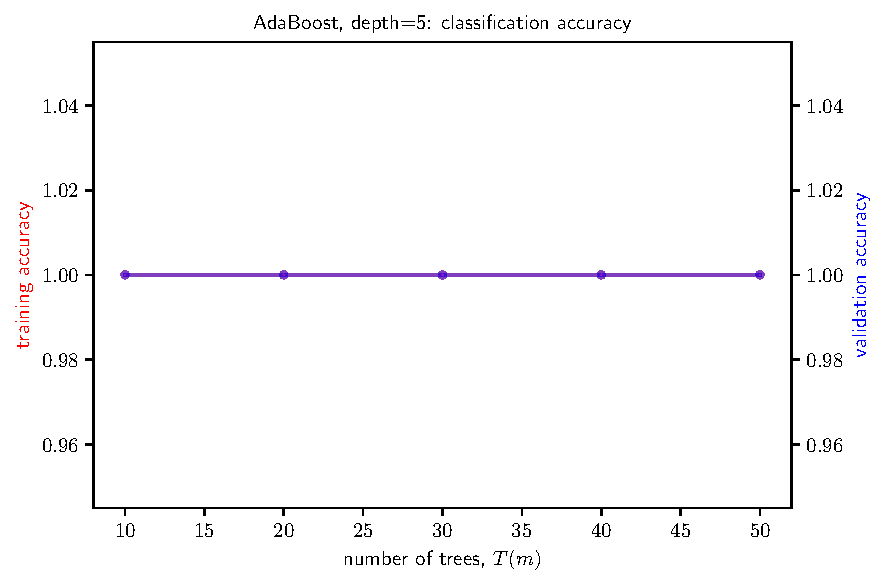
\includegraphics[width=0.6\linewidth]{figs/figadaboost_5_pt3_traindev.pdf}
  \caption{Adaboost: Train and validaition curves for $d_{\max}=5$}\label{fig3a3}
\end{figure}
}

\question{b}{
  For each $d_{\max}$ value, discuss what you believe is the dominating factor in the performance loss based on the concept of bias-variance decomposition. Can you suggest some alternative configurations of
  the ensemble that might lead to better performance for this data? Why do you believe so?
}
\answer{
  From the given Figures~\ref{fig3a1}-\ref{fig3a3}, we observe that for $d_{\max} = 1$, as $T$ increases, performance increases, and that the boosted model is of low bias, and low variance. Similarly, for $d_{\max} = 2$, the model is of lower bias, and lower variance, and performance improves faster to the optimum at $T=26$ compared to the previous $d_{\max} =1$ setting. For $d_{\max} = 5$, again the the model is of lower bias, and lower variance, and for all $T$ in the given set, performance converges faster to the optimum value of $100\%$ compared to the previous $d_{\max} =2$ setting.

  However, we observe that on the train and validation sets, it is possible that overtraining occurs: at $T>5$ taking $\sim3.3\,s$ for $d_{\max} = 5$, while for $d_{\max} = 2$, similar pattern is observed at $T>26$ taking $\sim5.4\,s$, and for $d_{\max} = 1$, this is observed at $T>110$ taking $\sim15.4\,s$. That is, it was observed that, there is no benefit or loss from adding more trees to the ensemble given these thresholds. In simple words, adding more trees past these thresholds make the ensemble bloated and increase computation time.

  Therefore, for this data-set, to obtain the best decision, in the fastest time possible, with the lowest performance loss, using $d_{\max} \in {1,2,5}$, the ensemble can be minimally configured using $T=5$ and $d_{\max} = 5$. This configuration was used for the \textbf{Kaggle Competition}.
  
  Generally, we observe that for \textbf{Adaboost}, the dominating factor in the low-bias low-variance performance is the number of trees $T$ in the ensemble, followed by the $d_{\max}$ of each tree.

 

}


\end{document}